\chapter{Esercizio 9}
Partendo dall'implementazione del processore, operante secondo il modello \texttt{IJVM}, si vuole
\begin{itemize}
    \item analizzare l'architettura mediante simulazione e fornire e approfondire lo studio per due funzioni; 
    \item modificare un codice operativo, documentando le modifiche effettuate.
\end{itemize}

\section{Il processore Mic-1}
Il processore Mic-1 è un utile esempio didattico con due scopi prinicpali:
\begin{enumerate}
    \item mostrare come sia possibile realizzare una microarchitettura che implementi un semplice set di istruzioni, usando elementi logici di base;
    \item mostrare come la realizzazione di un sistema, apparenemente complesso si  riduca in realtà alla progettazione di un'unità operatica e di unità di controllo.
\end{enumerate}

\noindent Il set di istruzioni implementato dal Mic-1 è un sottoinsieme di quello della \textit{Java Virtual Machine}, 
denominato \texttt{IJVM}, in quanto opera unicamente su interi.\\
La particolarità di tale processore èq eulla di non disporre di registri generali, basando la sua architettura sullo \textit{stack}:
infatti le varie istruzioni e logiche non hanno operandi espliciti, ma sono prelevati secondo la struttura \textit{last-in-first-out}.\\
L'implementazione di tale processore è detta in \textit{logica microprogrammata}: ciascuna 
istruzione \texttt{IJVM} è implemetata come una sequenza di microistruzioni, dette microprocedure; tali sequenze compongono il microprogramma, 
che è tipicamente memorizzato in una ROM interna al processore.

\subsection{Unità operativa}
L'unità operatia del processore è composta da ALU, i suoi ingressi e le sue uscite.
\begin{figure}[H]
	\centering
	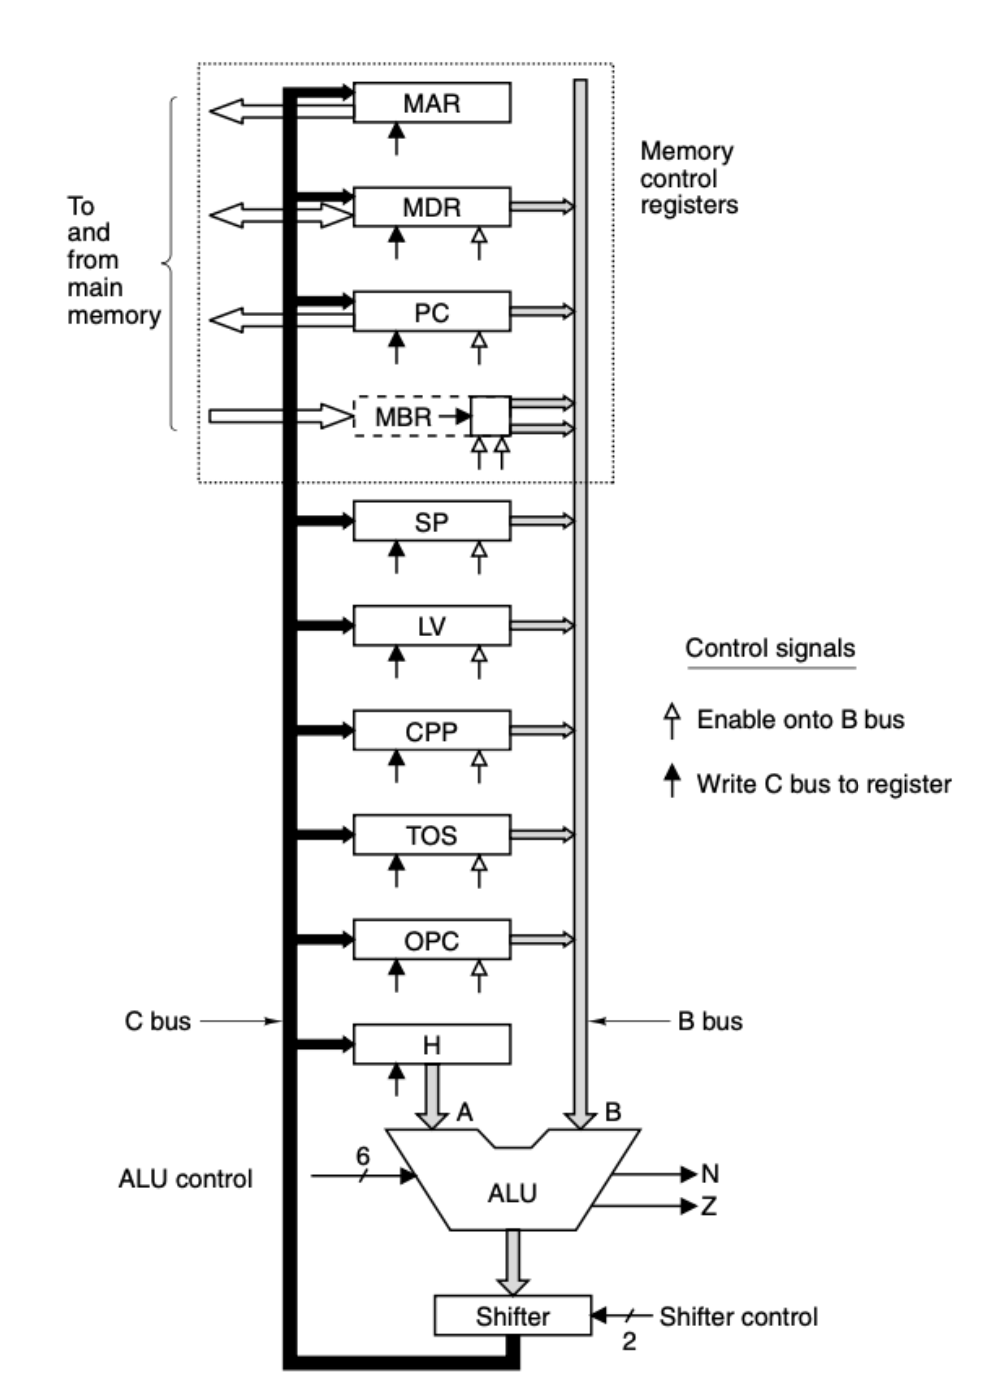
\includegraphics[width=0.8\textwidth]{img/Esercizio_9/uo_mic-1}
	\caption{Unità operativa del Mic-1}
	\label{uo_mic-1} 
\end{figure}
\noindent Ogni registro ha dimensione di 32 bit e non è accessibile dal programmatore, ma solo dal microprogramma.\\
Vi sono due bus, \texttt{B} e \texttt{C}, collegati rispettivamente al secondo ingresso e all'uscita dell'ALU; il primo ingresso dell'ALU è invece collegato esclusivamente al registro \texttt{H} (\textit{holding}).\\
Alcuni registri sono cablati in modo da poter essere usati solo per uno scopo specifico:
\begin{itemize}
    \item registri dell'interfaccia con la memoria 
    \begin{itemize}
        \item \texttt{MAR}: memory address register;
        \item \texttt{MDR}: memory data register;
        \item \texttt{PC}: program counter;
        \item \texttt{MBR}: memory byte register;
    \end{itemize}
    \item registro che mantienre il primo operando dell'ALU
    \begin{itemize}
        \item \texttt{H}: holding.
    \end{itemize}
\end{itemize}

\subsection{Microistruzioni}
Per controllare l'unità operativa del processore, sono necesaari 29 segnali:
\begin{itemize}
    \item 9 segnali per controllare la scrittura dei dati dal bus \texttt{C} ai registri;
    \item 9 segnali per controlare quale registro è collegato al bus \texttt{B} e va in ingresso all'ALU;
    \item 8 segnali per controllare l'ALU;
    \item 2 segnali per abilitare lettura/scrittura sull'interfaccia \texttt{MAR}/\texttt{MDR};
    \item 1 segnale per abilitare il fetch sull'interfaccia \texttt{PC}/\texttt{MBR}
\end{itemize}

\subsection{Unità di Controllo}
L'unità di controllo del Mic-1 si comporta come un \textit{sequencer}, producendo in ciascun ciclo:
\begin{enumerate}
    \item lo stato dei segnali di controllo
    \item l'indirizzo della prossima microistruzione da eseguire
\end{enumerate}
Di seguito il diagramma completo del Mic-1:
\begin{figure}[H]
	\centering
	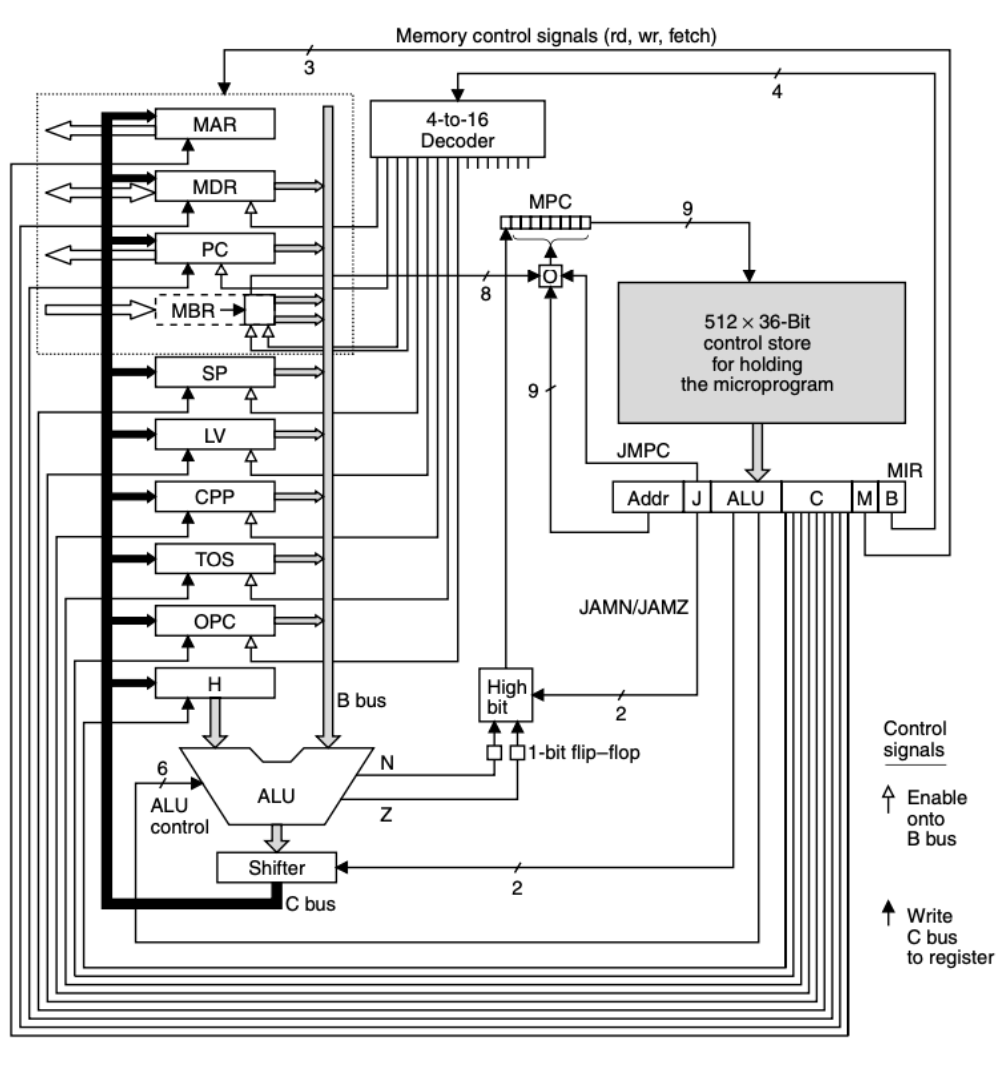
\includegraphics[width=0.8\textwidth]{img/Esercizio_9/diag_mic-1}
	\caption{Diagramma completo del Mic-1}
	\label{diag_mic-1} 
\end{figure}

\section{La microistruzione \texttt{ISUB}}
La microistruzione \texttt{ISUB} altro non è che la sottrazione di due operandi.\\
Per implementare l'instruzione, viene utilizzato linguaggio MAL, \textit{MicroAssembly Lenguage}, il quale viene convertito dal \textit{microassemblatore}.
L'istruzione è definita come segue
\begin{listing}[h]
    \caption{ISUB}
    \AtBeginEnvironment{minted}{%
    \renewcommand{\fcolorbox}[4][]{#4}}
    \begin{minted}[bgcolor=white, linenos]{dasm16}
    isub = 0x5C:
        MAR = SP = SP - 1; rd
        H = TOS
        MDR = TOS = MDR - H; wr; goto main
    \end{minted}
\end{listing}
L'indirizzo \texttt{0x5C} indica l'indirizzo in memoria della prima istruzioni da eseguire. Le restanti sono scritte nei registri successivi. \\
In tale istruzione si ha come prima istruzione quella di decrementare l' \texttt{SP}, ovvero lo \textit{stack pointer}, poiché nella fase iniziale punta alla testa dello stack, che può essere richiamta tramite \texttt{TOS}, \textit{Top of Stack}.
Inoltre l'indirizzo viene salvato nel \texttt{MAR}, \textit{Memory Address Register} e viene chiamata la funzione di read, \texttt{rd}.\\
Nella seconda operazione si preleva la testa dello stack tramite \texttt{TOS} e lo si memorizza nel registro \texttt{H}. \\
Recuperati gli operandi, si effettua l'operazione tra il dato \texttt{MDR}, \textit{Memory Data Register}, e \texttt{H}; si memorizza il risultato con l'istruzione \texttt{wr} nel \texttt{MDR}.\\
Per caricare l'istruzione nella memoria RAM del processore, si modifica il file \texttt{program.ajvm} e lo si compila:
\begin{listing}[h]
    \AtBeginEnvironment{minted}{%
    \renewcommand{\fcolorbox}[4][]{#4}}
    \begin{minted}[bgcolor=white, linenos]{dasm16}
    .main
    .var
    a
    .endvar
    BIPUSH 0xE
    BIPUSH 0xA
    ISUB
    ISTORE a
    HALT
    .endmethod
    \end{minted}
    \caption{ISUB - program.ajvm}
\end{listing}
dove tramite \texttt{BIPUSH} si caricano gli operandi nello stack, \texttt{ISUB} effettua l'operazione e \texttt{ISTORE} memorizza il risultato nella variabile.
\subsection{Simulazione}
Per eseguire la compilazione e quindi modificare il \texttt{control\_store} e la \texttt{ram}, si eseguono i seguenti comandi:
\begin{figure}[H]
	\centering
	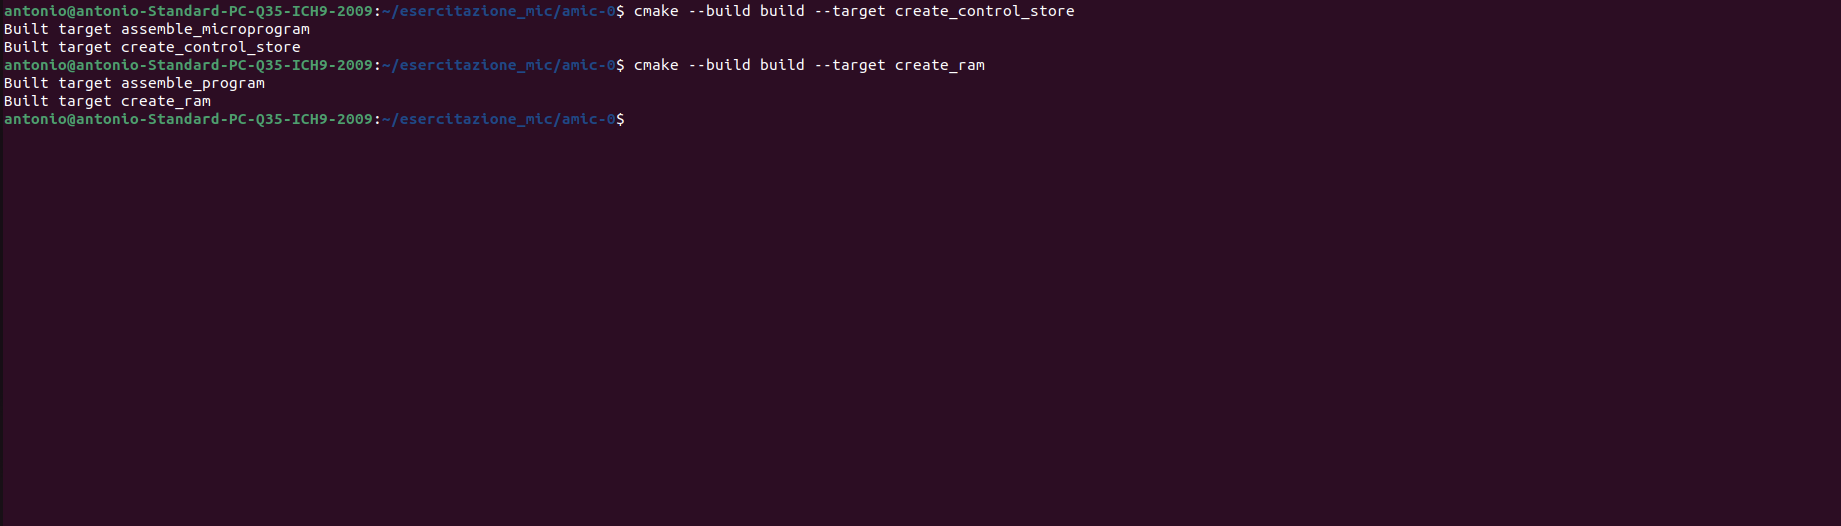
\includegraphics[width=0.8\textwidth]{img/Esercizio_9/Compile}
	\caption{Compilazione Control Store e RAM}
	\label{compile}
\end{figure}
Un modo per verificare che la compilazione è andata a buon fine, si può controllare come è modificata la RAM:
\begin{figure}[H]
	\centering
	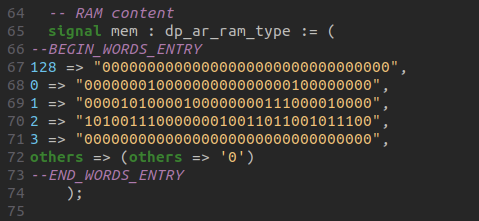
\includegraphics[width=0.8\textwidth]{img/Esercizio_9/ram_sub}
	\caption{Istruzione caricata nella RAM}
	\label{tam_sub}
\end{figure}
Si nota infatti che in corrispondenza della istruzione 1 si ha una stringa di 32 bit che altro non è la concatenzazione del primo dato, l'indirizzo dell'istruzione \texttt{BIPUSH}, il secondo dato e di nuovo l'indirizzo dell'istruzione \texttt{BIPUSH}. 
Nell'istruzione 2 si ha l'indirizzo dell'operazione \texttt{ISUB} e quella di \texttt{ISTORE}.\\
Si può a questo punto effettuare il testbench (ovviamente è stato modificato opportunamente il file \texttt{processor\_tb.vhd}):
\begin{figure}[H]
	\centering
	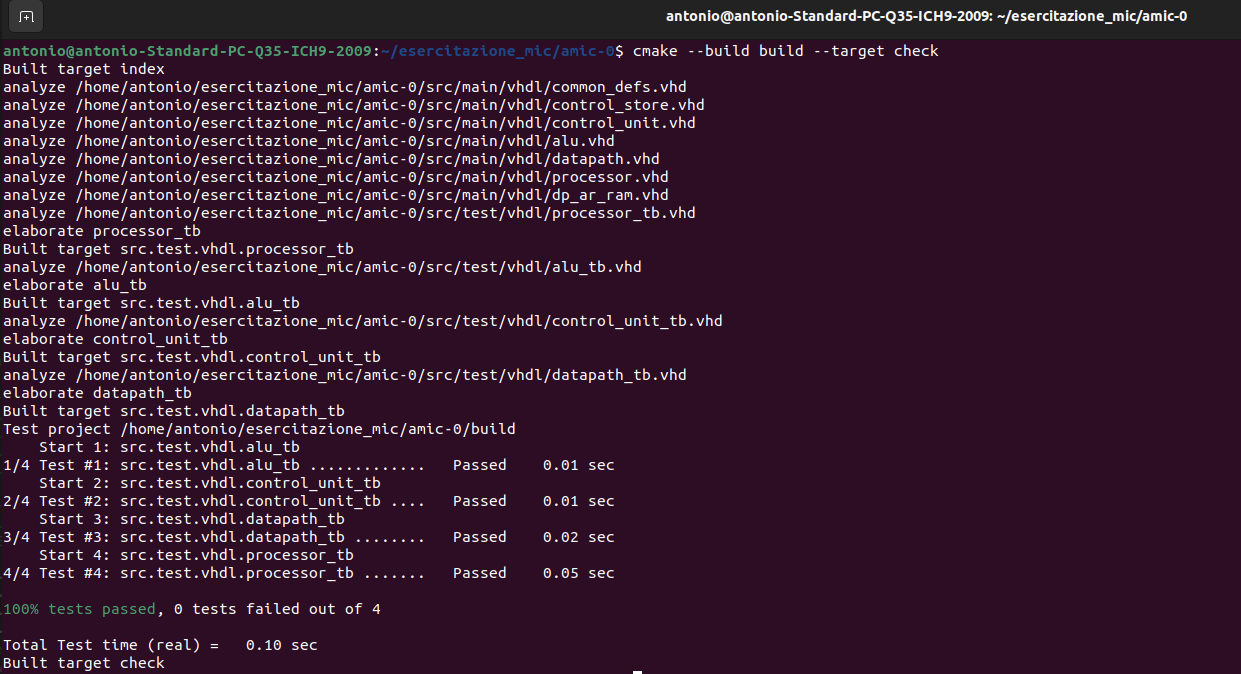
\includegraphics[width=0.8\textwidth]{img/Esercizio_9/tb_sub}
	\caption{Testbench ISUB}
	\label{tb_sub}
\end{figure}
e questa è la seguente onda risultante
\begin{figure}[H]
	\centering
	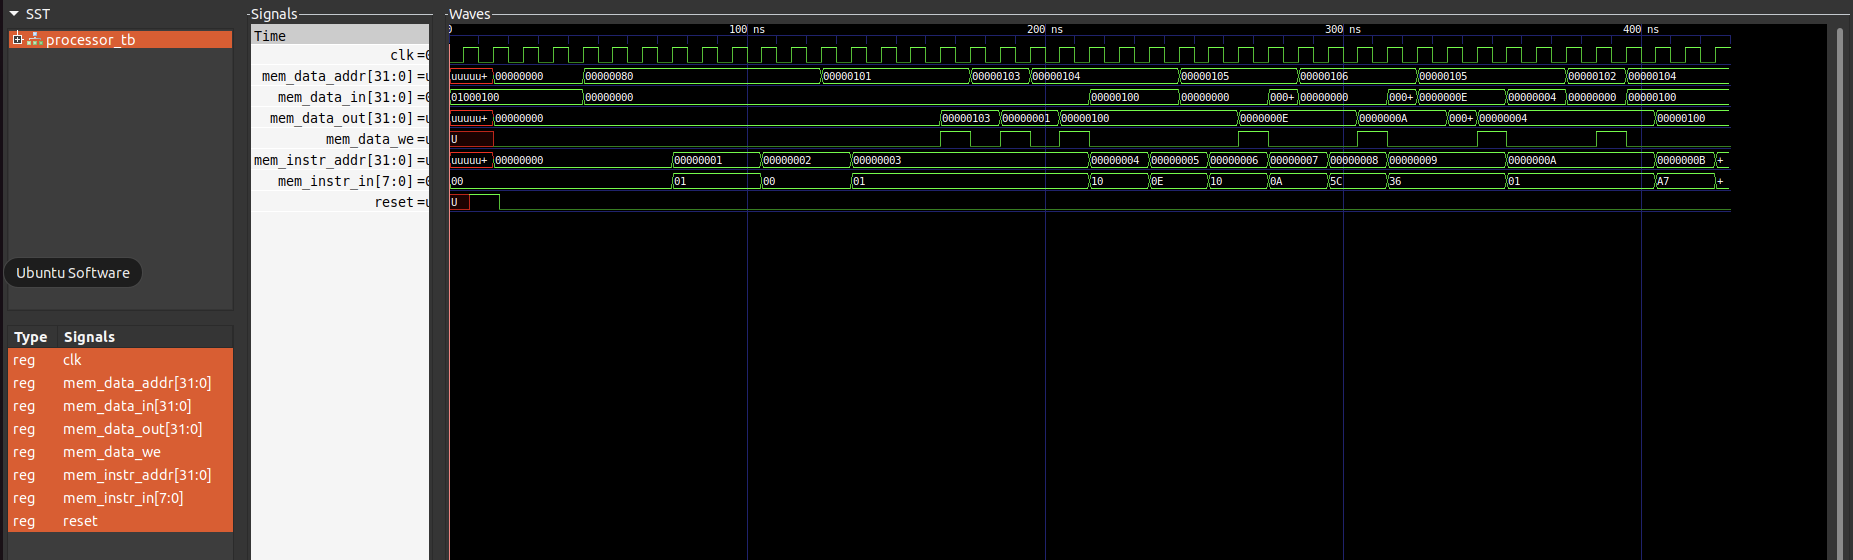
\includegraphics[width=0.8\textwidth]{img/Esercizio_9/sub_wave}
	\caption{Onda ISUB}
	\label{sub_wave}
\end{figure}